\chapter{Link Budget}

\begin{figure}[H]
\centering
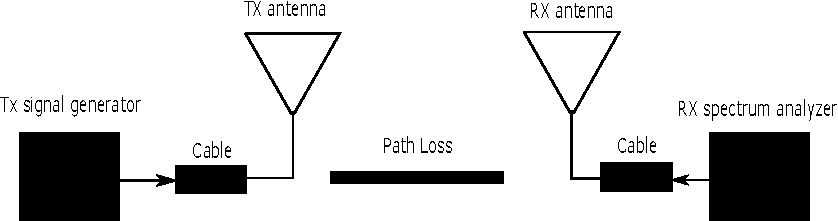
\includegraphics[width=0.7\textwidth]{link_budget_illu.pdf}
\caption{Link budget illustration}
\label{dijdkkfkf}
\end{figure}


%As seen on the Figure above an important aspect for the link 





%A Link budget, takes into account all the losses and gains from the transmitter antenna to the receiver antenna. 
A link budget is calculated to find the loss though the whole system, so the needed transmission power is found or the needed antenna gain is found, for a specific transmission power.

%A Link budget is calculated to take into account the attenuation of the transmitted signal due to propagation, which depends on the circumstances like reflections, free-space loss ,buildings etc. other factors included are cable loss, antenna gains, polarization loss. %which depends if the transmitter antenna and the receiver antenna a pointing directly at each other, if not some loss will occur  etc. 
Such a calculation is given as:

\begin{equation}
P_{RX} = P_{TX} + G_{TX} - L_{TX} - L_{PL} - L_{MISC} + G_{RX} - L_{RX}
\label{link_calc}
\end{equation}

\begin{where}
\va{$P_{RX}$}{Power Received}{dBm}
\va{$P_{TX}$}{Power transmitted}{dBm}
\va{$G_{TX}$}{Transmitter antenna gain}{dBi}
\va{$L_{TX}$}{Transmitter losses (cable,coax)}{dB}
\va{$L_{PL}$}{Path Loss}{dB}
\va{$L_{MISC}$}{misc losses(polarization losses, other losses)}{dB}
\va{$G_{RX}$}{Receiver antenna gain}{dBi}
\va{$L_{RX}$}{Receiver losses (cable,coax)}{dB}
\end{where}
\newpage
\subsection{Polarization loss factor (PLF)}
Polarization loss as plays a factor in the Link Budget calculation. There is Linear Polarization, Circular Polarization. For Linear polarization the antenna can be turned horizontal and vertical direction this is illustrated in the following Figure:

\begin{figure}[H]
\centering
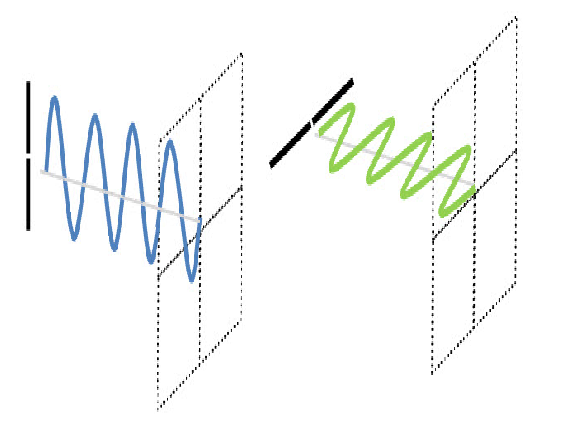
\includegraphics[width=0.4\textwidth]{polariz_ver_hor_lin.pdf}
\caption{Linear horizontal and vertical polarization}
\label{fig:pol_ver_hor}
\end{figure} 

The PLF for Linear Polarized antennas can be calculated by the equations given on the following Figure depending on the angle of the the antennas, an illustration of the PLF for max, non and signal loss with dependence on an angle:

\begin{figure}[H]
\centering
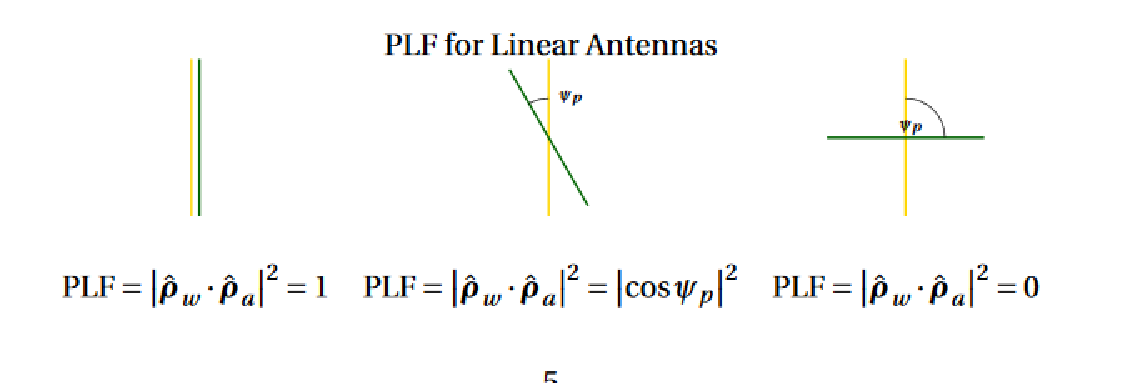
\includegraphics[width=0.6\textwidth]{plf.pdf}
\caption{Minimum, maximum and PLF loss depending on the angle}
\label{fig:lin_plf}
\end{figure} 

As it can be seen if the two antennas are pointing directly at each other with the same polarization there will be no PLF. While if one antenna is vertically polarized and the other is horizontally polarized, then no power will be transferred. While there will be some power loss if the two antennas are not $100\%$ polarized, meaning there is an polarization miss match ,there will be some power loss depending on the angle.

\subsubsection{PLF loss calculated}

For the measurements conducted the PLF factor is calculated with an angle $\psi$ of 5$^{\circ}$, as the two antennas are not pointing directly at each other, this gives the following PLF loss factor:

\begin{equation}
cos(\psi)^{2} = cos(5)^2 = 0.9962
\end{equation}

Then to get it in dB:

\begin{equation}
10 \cdot log(0.9962) = -0.0381dB
\end{equation}



%the angle of the antennas as they are not pointing directly at each other is around  5$^{\circ}$


\subsection{Cable Loss}
As a part of the Link Budget cable loss is also included. The cable loss is depended on the length of the cable, where the longer the cable the more cable loss there will be as the signal will lose travelling strength through the cable. Where for each cable it is indicated in the data sheet how much power is lost per meter at different frequencies, this is different for each type of cable. 


\subsubsection{Calculated cable loss}
Two different types of cables where used these are:

\begin{itemize}
\item rg223/u 
\item SUCOFLEX$\_$104
\end{itemize}

The length for the  rg223/u cable is of 1M, while for the SUCOFLEX$\_$104 cable, two SUCOFLEX$\_$104 cables where used with different lengths of 1.5m and 2.20m.

The cable loss for the rg223/u cable is read from the data sheet then interpolated, from the data sheet it is given that the attenuation factor is given in dB per 100 meters. 

%\begin{equation}
%Attenuation factor = [dB/100]
%\end{equation}

In the data sheet it can be read that for 1000 Mhz a loss of  13.4dB per 100 m, while for 3 Ghz it is 24.8dB per 100 m. There has been made an interpolation of the Attenuation factors, so that a more precise Attenuation factor can be calculated so for 2.58 Ghz and 856 Mhz the following Attenuation factors have been calculated, for 1 m:

\begin{equation}
Attenuation factor\_2.58 = \frac{22.4}{100}  = 0.224dB
\end{equation}

\begin{equation}
Attenuation factor\_858 = \frac{12.7}{100}  = 0.127dB
\end{equation}

While for the SUCOFLEX$\_$104 cable the following formula has been used to calculate the Attenuation factor, for both 1.5m and 2.20m:

\begin{equation}
a_{25} = a\cdot \sqrt{f(Ghz)} + b \cdot f(Ghz) \quad [db/m]
\end{equation}

\begin{where}
\va{$a$}{Nom.attenuation = 0.2291}{-}
\va{$b$}{Nom.attenuation = 0.0071}{-}
\end{where}

The attenuation factor for 858 Mhz is equal to 0.327dB while for 2.58 Ghz it is 0.579dB for 1.5m. While for 2.20m the attenuation factor for 858 Mhz is equal to 0.480dB, while for 2.58 Ghz it is 0.850dB. In the following an Table of the cable loss can be seen: 
\\
\\
\begin{table}[H]
\centering
\caption{Cable loss table}
\label{my-label}
\begin{tabular}{|l|l|l|l|l|l|}
\hline
                                                                            & \begin{tabular}[c]{@{}l@{}}Mono \\ 2.58 Ghz\end{tabular} & \begin{tabular}[c]{@{}l@{}}Mono \\ 858 Mhz\end{tabular} & \begin{tabular}[c]{@{}l@{}}Patch \\ 2.58Ghz\end{tabular} & \begin{tabular}[c]{@{}l@{}}Patch \\ 858Mhz\end{tabular} & \begin{tabular}[c]{@{}l@{}}Demo board \\ 868 Mhz\end{tabular} \\ \hline
Cable loss: rg223\_u                                                        & -0.224dB                                                 & -0.127dB                                                & -0.224dB                                                 & -0.127dB                                                & -                                                             \\ \hline
\begin{tabular}[c]{@{}l@{}}Cable loss: SUCOFLEX\_104 \\ (1.5m)\end{tabular} & -0.579dB                                                 & -0.327dB                                                & -0.579dB                                                 & -0.327dB                                                & -                                                             \\ \hline
\begin{tabular}[c]{@{}l@{}}Cable loss: SUCOFLEX\_104 \\ (2.5m)\end{tabular} & -0.850dB                                                 & -0.480dB                                                & -0.850dB                                                 & -0.480dB                                                & -                                                             \\ \hline
Cable loss: Demoboard                                                       &                                                          & -                                                       & -                                                        & -                                                       & -2dB                                                          \\ \hline
Total Loss                                                                  & -1.6530dB                                                &                                                         & -1.6530dB                                                 & -0.9340dB                                              & -2dB                                                          \\ \hline
\end{tabular}
\end{table}

%The Antenna Efficiency is measured in Satimo lab, which gives an Antenna Efficiency txt. file where the Antenna Efficiency for the given frequency is specified and multiplied with 2 as there are two antennas.  


\subsection{LOS, nLOS and NLOS}

Other factors to consider when calculating a link budget is if there is \textbf{Line-Of-Sight(LOS)}, which means that if there is an obstacle in between the transmitter antenna and the receiver antenna it does not block the signal, as the two antennas can see each other, this is illustrated on the following Figure:

\begin{figure}[H]
\centering
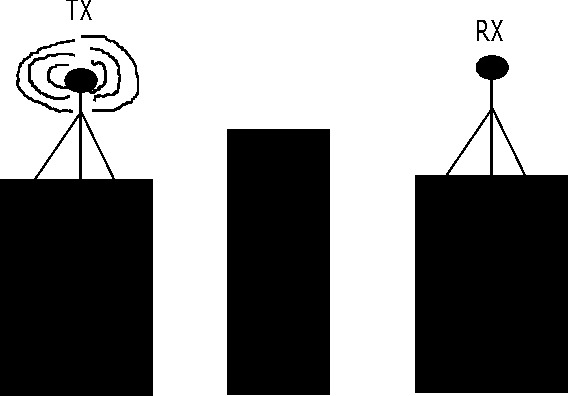
\includegraphics[width=0.35\textwidth]{los.pdf}
\caption{LOS illustration}
\label{LOS}
\end{figure}  


Where the counter-part is \textbf{Non-Line-Of-Sight(NLOS)}, which means that the path is interfered, which could be by a building standing in-between the transmitter antenna and the receiver antenna, where the two antennas cannot see each other, this is illustrated on the following Figure: 

\begin{figure}[H]
\centering
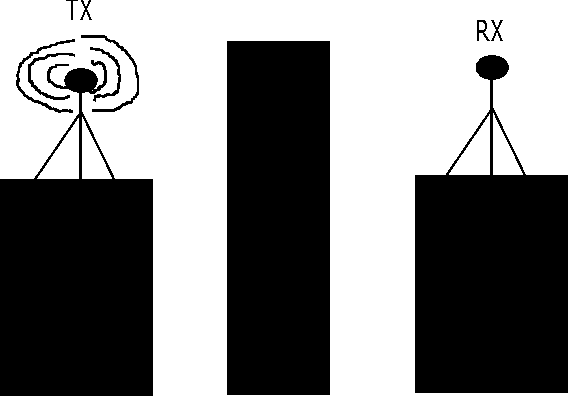
\includegraphics[width=0.35\textwidth]{nlos.pdf}
\caption{NLOS illustration}
\label{dijdkkfkfddd}
\end{figure} 

Another one is \textbf{Near Line Of Sight(nLOS)}, which means that the path is partially interfered,  which could be by a building. Which is illustrated on the following Figure:

\begin{figure}[H]
\centering
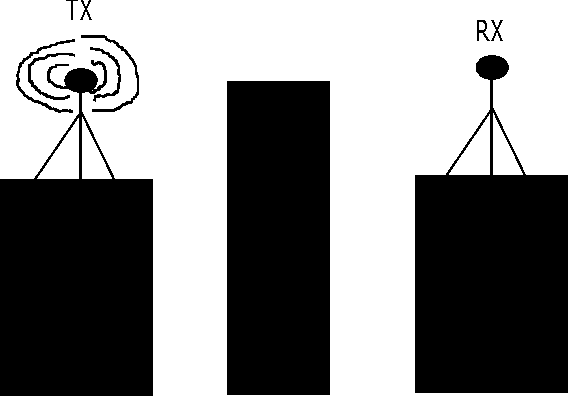
\includegraphics[width=0.35\textwidth]{nearlos.pdf}
\caption{nLOS illustration}
\label{nLOS}
\end{figure} 


The different Line-Of-Sights, play a big factor when considering the Fresnel Zones which is further explained in Chapter \ref{fres_zone}, which also plays a big part in the received Power. As explained in the Fresnel Zone chapter there must be $60\%$ clearance in the first Fresnel zone, as the strongest signals are in the first Fresnel zone ,this could be a problem if there is too much \textbf{NLOS}, as the antennas would need to be risen higher.       







%interpolation 

%1M - rg223/u  22.41/100  = 0.224dB for 2.58 Ghz
%1M - rg223/u  12.7/100  =  0.127dB for 856  Mhz


%1.5M - SUCOFLEX_104 - attenuation factor_858  * 1.5 = 0.218 dB/M * 1.5M = 0.327dB  
%1.5M - SUCOFLEX_104 - attenuation factor_2.58 * 1.5 = 0.2386 dB/M * 1.5M = 0.579dB 

%2.20M - SUCOFLEX_104 - attenuation factor_858  * 2.20 = 0.218 dB/M  * 2.20M = 0.480dB
%2.20M - SUCOFLEX_104 - attenuation factor_2.58 * 2.20 = 0.2386 dB/M * 2.20M = 0.850dB




%If there is \textbf{NLOS}, shadowing must also then be considered as a part of the Link budget.
%\\
%\\
%Another thing to consider when, expecting the Power received is the Fresnel Zone which is further explained in Chapter \ref{fres_zone}    


